\documentclass{standalone}
\usepackage{tikz}
\usepackage{tikz-timing}
\usetikzlibrary{circuits.logic.US}
\tikzstyle{branch}=[fill,shape=circle,minimum size=2pt,inner sep=0pt]
\begin{document}
\begin{tikztimingtable}
A         & LLL HHL LLL LHH LLL \\
B         & LLL LHH LLL HHL LLL \\
C         & LLL LHL LLL LHL LLL \\
D         & HHH LLL HHH LLL HHH \\
E         & LLL HLL LLL LLH LLL \\
F         & LLL LLH LLL HLL LLL \\
Pulse     & LLL LHH LLL LHH LLL \\
Direction & LLL LLH HHH HHL LLL \\
\end{tikztimingtable}
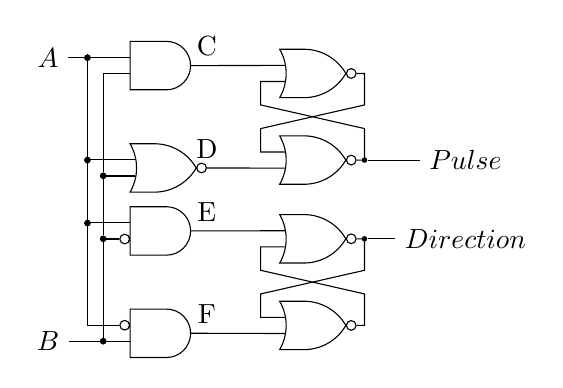
\begin{tikzpicture}[circuit logic US]
\node (A) at (0,1.8) {$A$};
\node (B) at (0,-1.8) {$B$};
\node[branch, draw] at ($(A)+(0.5,0)$) (A1) {};
\node[branch, draw] at ($(A1)+(0,-1.3)$) (A2) {};
\node[branch, draw] at ($(A2)+(0,-0.8)$) (A3) {};
\node[branch, draw] at ($(B)+(0.7,0)$) (B1) {};
\node[branch, draw] at ($(B1)+(0,+1.3)$) (B2) {};
\node[branch, draw] at ($(B2)+(0,+0.8)$) (B3) {};
\node[and gate, draw, inputs=ni] at ($(B2) +(0.7,+0.1)$) (And1) {};
\node[and gate, draw, inputs=in] at ($(B1) +(0.7,+0.1)$) (And2) {};
\node[and gate, draw, inputs=nn] at ($(A1) +(0.9,-0.1)$) (And3) {};
\node[nor gate, draw, inputs=nn] at ($(A2) +(0.9,-0.1)$) (Nor1) {};
\node[nor gate, draw, inputs=nn] at ($(And1) +(1.9,-0.1)$) (Nor2) {};
\node[nor gate, draw, inputs=nn] at ($(And2) +(1.9,+0.1)$) (Nor3) {};
\node[nor gate, draw, inputs=nn] at ($(Nor1) +(1.9,+0.1)$) (Nor4) {};
\node[nor gate, draw, inputs=nn] at ($(And3) +(1.9,-0.1)$) (Nor5) {};
\node (P) at ($(Nor4)+(2,0)$) {$Pulse$};
\node (D) at ($(Nor2)+(2,0)$) {$Direction$};
\draw (A) -- (A1);
\draw (B) -- (B1);
\draw (A1) -- (A2);
\draw (A2) -- (A3);
\draw (B1) -- (B2);
\draw (B2) -- (B3);
\draw (A3) |- (And1.input 1);
\draw (B2) |- (And1.input 2);
\draw (A3) |- (And2.input 1);
\draw (B1) |- (And2.input 2);
\draw (A1) |- (And3.input 1);
\draw (B3) |- (And3.input 2);
\draw (A2) |- (Nor1.input 1);
\draw (B3) |- (Nor1.input 2);
\draw (And1.output) -- +(0.2,0) node[above]{E} -- (Nor2.input 1);
\draw (And2.output) -- +(0.2,0) node[above]{F} -- (Nor3.input 2);
\draw (Nor2.output) -| node[branch] (D1) {} +(0.1,-0.4) -- ($(Nor3) +(-0.6,+0.4)$) |- (Nor3.input 1);
\draw (Nor3.output) -| +(0.1,0.4) -- ($(Nor2) +(-0.6,-0.4)$) |- (Nor2.input 2);
\draw (D1) -- (D);
\draw (And3.output) -- +(0.2,0) node[above]{C} -- (Nor5.input 1);
\draw (Nor1.output) -- +(0,0) node[above]{D} -- (Nor4.input 2);
\draw (Nor5.output) -| +(0.1,-0.4) -- ($(Nor4) +(-0.6,+0.4)$) |- (Nor4.input 1);
\draw (Nor4.output) -| node[branch] (P1) {} +(0.1,0.4) -- ($(Nor5) +(-0.6,-0.4)$) |- (Nor5.input 2);
\draw (P1) -- (P);
\end{tikzpicture}
\end{document}
